\documentclass[../Languages.tex]{subfiles}

\begin{document}
\usec{Ruby}\label{sec:ruby}

\cd{Ruby} is a dynamic, reflective, object-oriented, general-purpose
programming language. It was designed and developed in the mid-1990s by
Yokihiro ``Matz'' Matsumoto in Japan.

According to its creator, \cd{Ruby} was influenced by \cd{Perl},
\cd{Smalltalk}, \cd{Eiffel}, \cd{Ada}, and \cd{Lisp}. It supports multiple
programming paradigms, including functional, object-oriented, and imperative.
It also has a dynamic type system and automatic memory management.

\subsection{Influence}\label{sub:influence}

\begin{Figure}
  \centering
  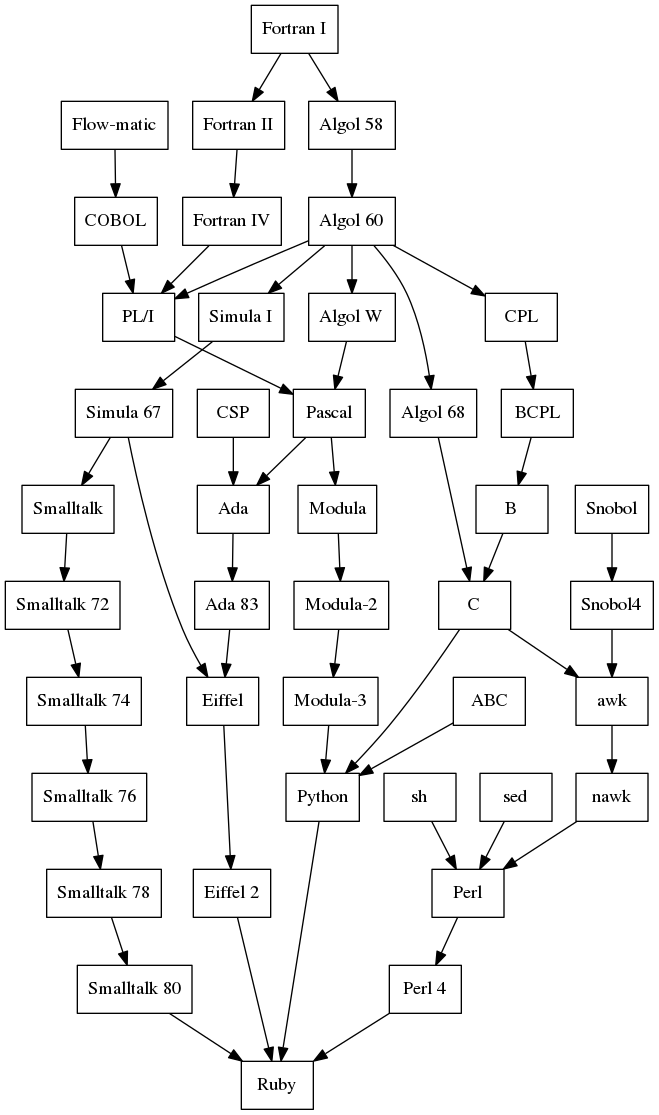
\includegraphics[height=0.5\textheight]{ruby}
  \captionof{figure}{Inheritance diagram for \cd{Ruby}.}
\end{Figure}

\newpage
\end{document}
